\chapter{Architecture Logicielle et Conception Système}
\label{chap:archi_conception}

\section{Principes Directeurs d'Ingénierie Logicielle}

Le système CBIR est conçu selon les principes de la \textbf{Clean Architecture} organisée en un \textbf{Monolithe Modulaire}. Ce modèle garantit une séparation stricte des préoccupations (\textit{Separation of Concerns}) tout en évitant les surcoûts d'orchestration réseau propres aux micro-services distribués lors de la manipulation de flux vectoriels denses.

\begin{figure}[H]
    \centering
    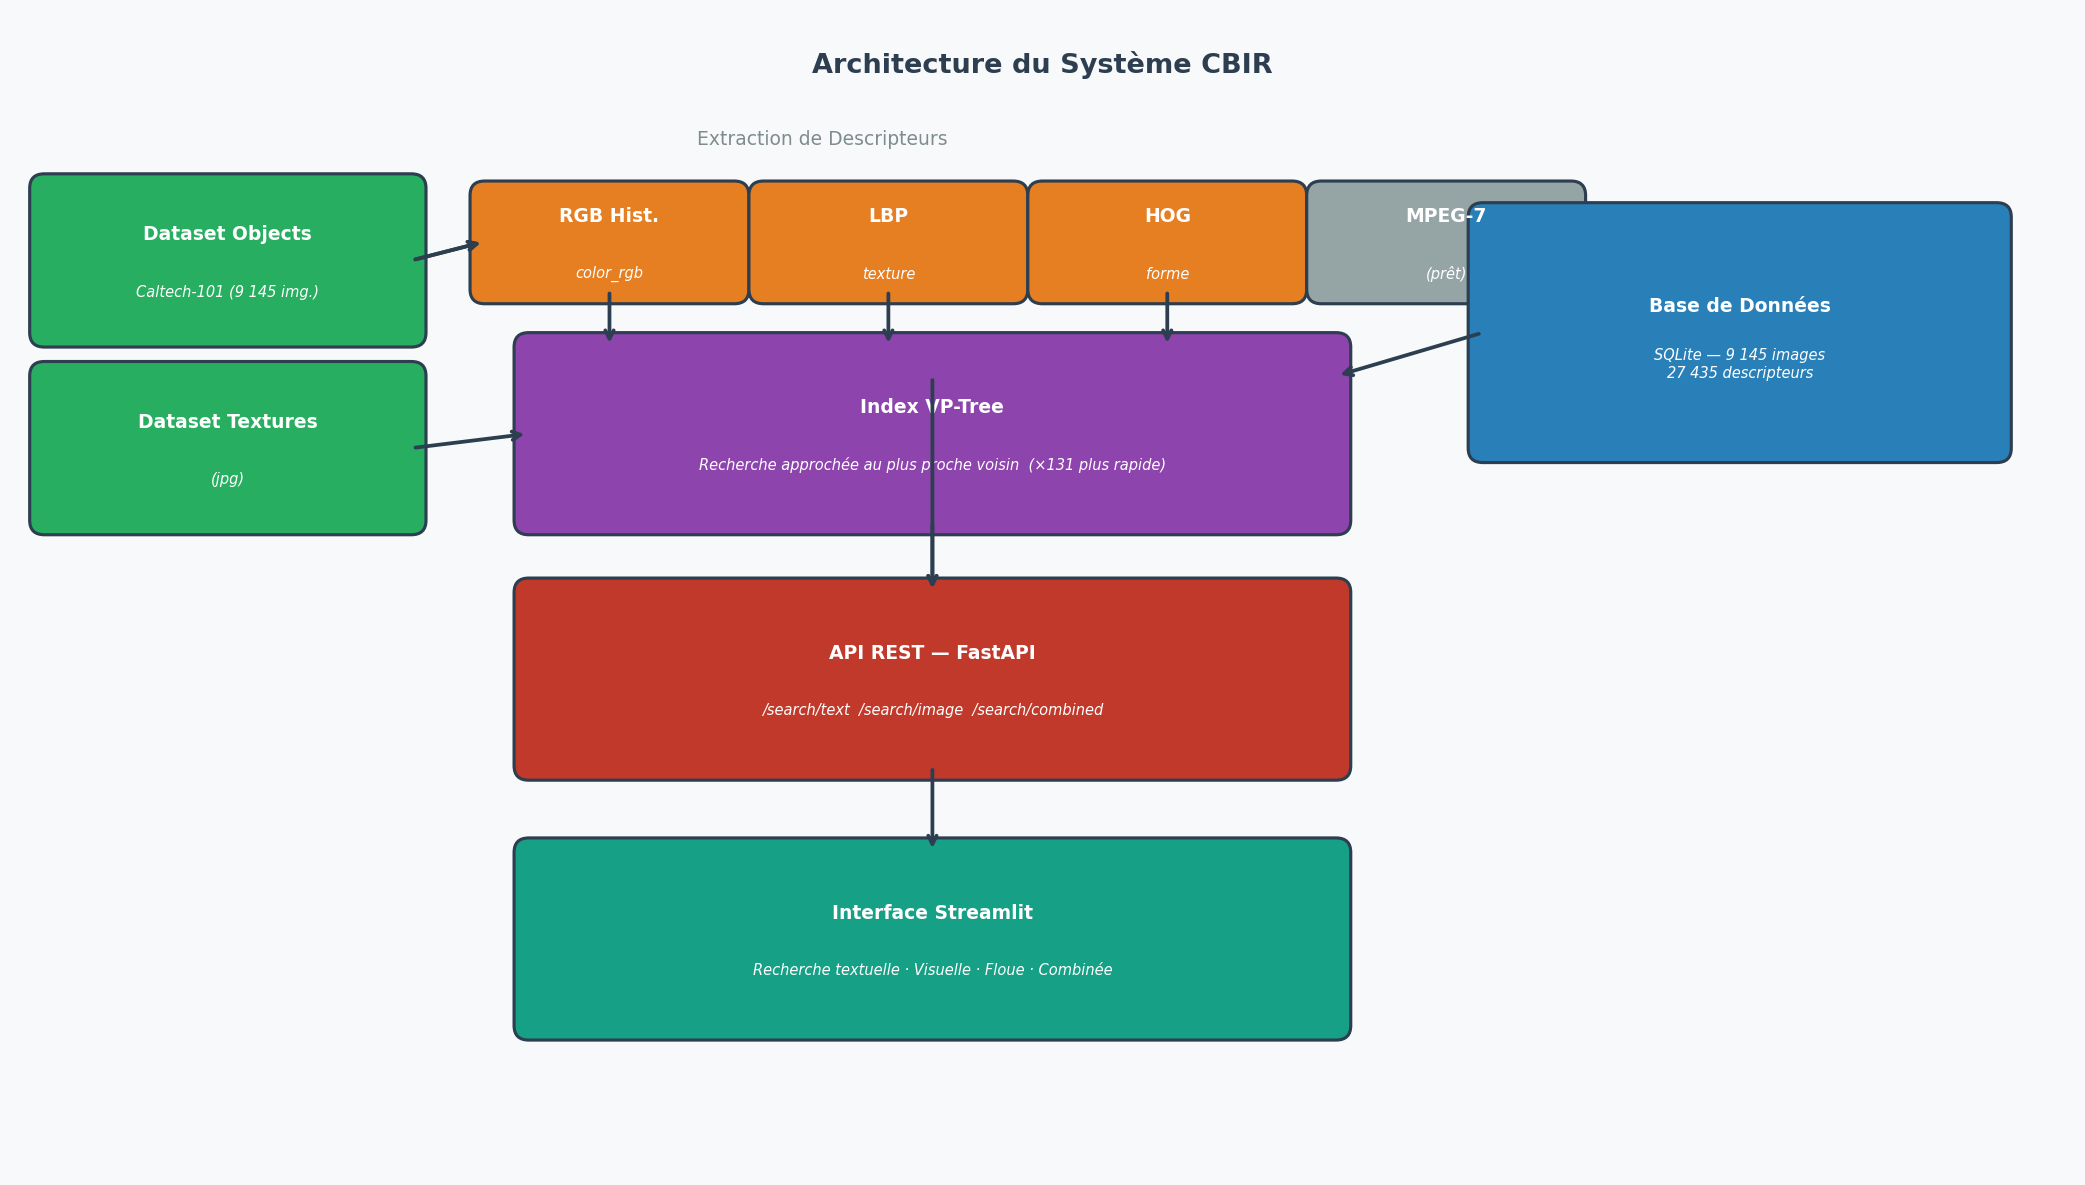
\includegraphics[width=0.90\textwidth]{figures/architecture.png}
    \caption{Architecture modulaire du système CBIR : flux des données depuis les sources brutes jusqu'à l'interface Streamlit.}
    \label{fig:archi_principale}
\end{figure}

Le découpage applicatif comprend six couches étanches :
\begin{enumerate}[nosep]
    \item \textbf{Configuration (\texttt{cbir/config.py}) :} Gestion immuable des variables d'environnement via \texttt{pydantic-settings} et fichier \texttt{.env}.
    \item \textbf{Persistance relationnelle (\texttt{cbir/database.py}) :} Opérations ACID sous SQLite via gestionnaire de contexte.
    \item \textbf{Descripteurs visuels (\texttt{cbir/descriptors/}) :} Fabrique unifiée (\textit{Factory Pattern}) et extracteurs spécialisés (RGB, HSV, LBP, HOG, MPEG-7).
    \item \textbf{Espaces métriques et Indexation (\texttt{cbir/distances/} \& \texttt{cbir/indexing/}) :} Bibliothèque de distances vectorielles et moteur VP-Tree.
    \item \textbf{Moteur de recherche métier (\texttt{cbir/search.py}) :} Coordination de la recherche textuelle, floue, visuelle $k$-NN et fusion multimodale.
    \item \textbf{Exposition de services (\texttt{cbir/api.py} \& \texttt{frontend/app.py}) :} Serveur d'API REST asynchrone FastAPI et tableau de bord Streamlit.
\end{enumerate}

\section{Modélisation de la Base de Données Relationnelle}

La persistance des métadonnées applicatives est déléguée à \textbf{SQLite 3}. Le schéma normalisé en 3NF est composé de quatre tables maîtresses (figure \ref{fig:db_schema_compact}).

\begin{figure}[H]
    \centering
    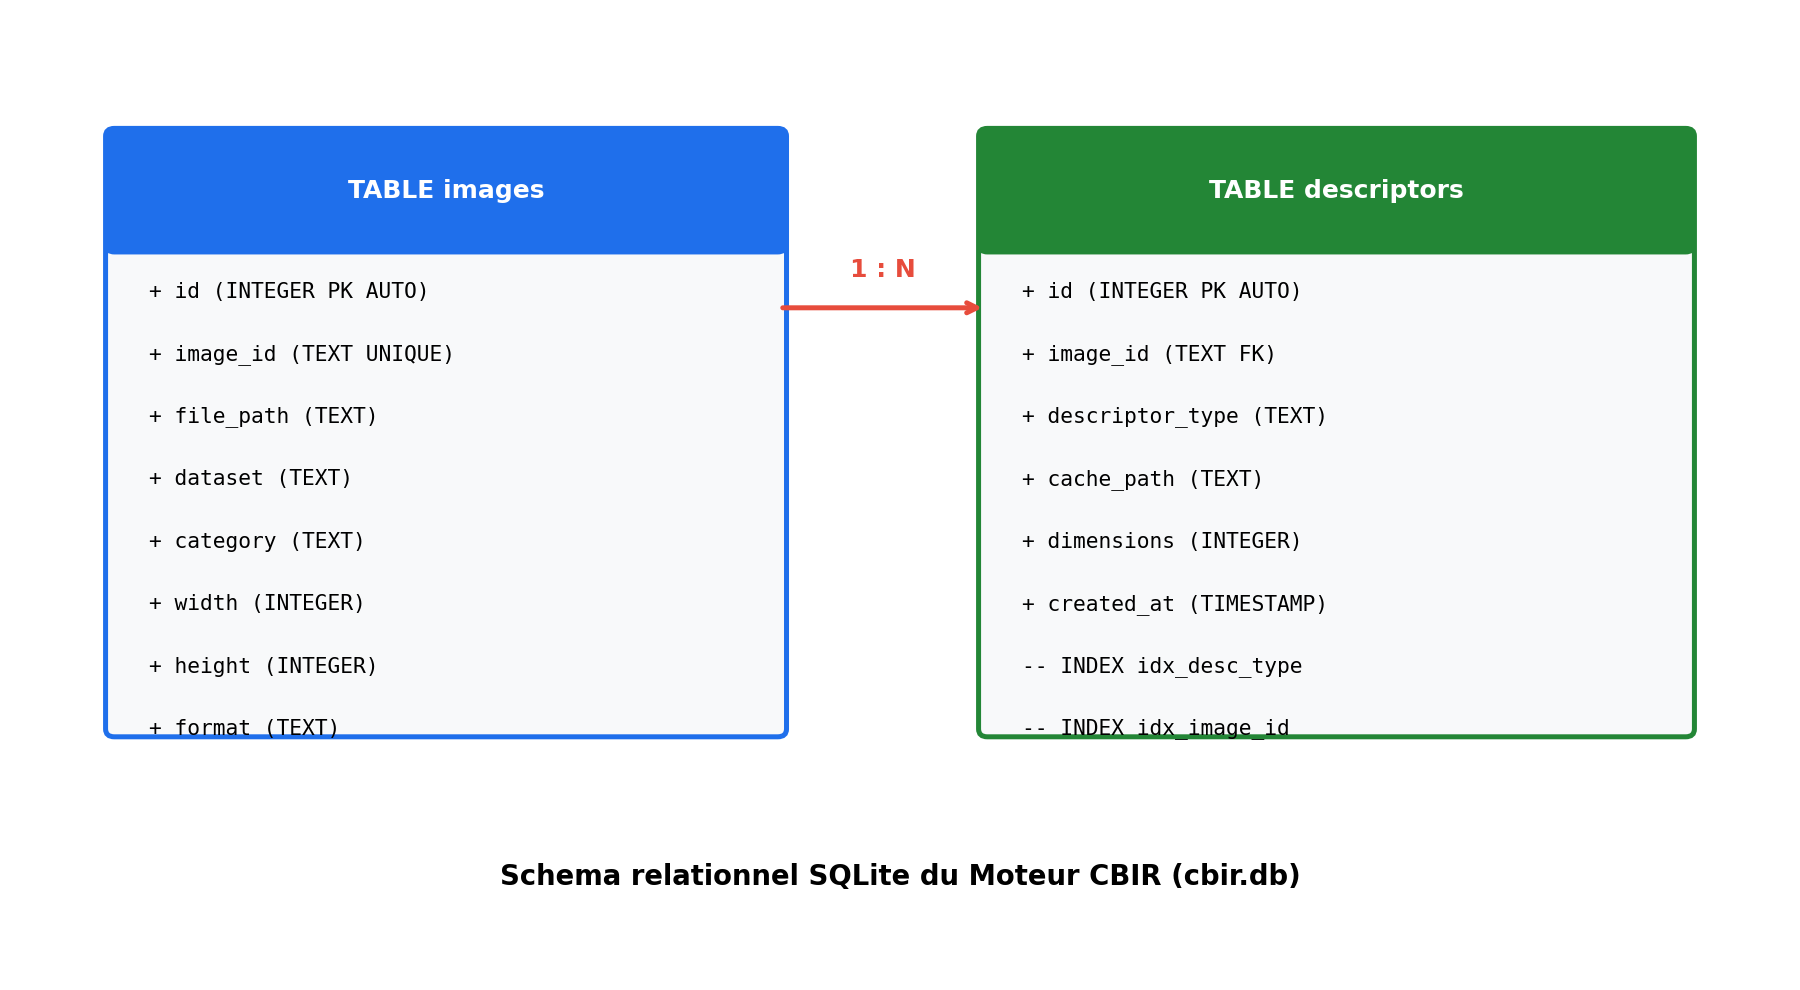
\includegraphics[width=0.85\textwidth]{figures/database_schema.png}
    \caption{Schéma entité-association de la base relationnelle \texttt{cbir.db}.}
    \label{fig:db_schema_compact}
\end{figure}

\begin{lstlisting}[language=SQL, caption={Extrait DDL des tables clés de cbir.db}]
CREATE TABLE IF NOT EXISTS images (
    id INTEGER PRIMARY KEY AUTOINCREMENT,
    image_id TEXT UNIQUE NOT NULL,       -- ex: "objects/butterfly/image_0001"
    file_path TEXT NOT NULL,
    dataset TEXT NOT NULL,               -- "objects" ou "textures"
    category TEXT NOT NULL,              -- "butterfly", "airplanes"...
    width INTEGER, height INTEGER,
    format TEXT DEFAULT 'JPEG',
    indexed_at TIMESTAMP DEFAULT CURRENT_TIMESTAMP
);
CREATE INDEX IF NOT EXISTS idx_images_cat ON images(category);
CREATE INDEX IF NOT EXISTS idx_images_id ON images(image_id);

CREATE TABLE IF NOT EXISTS descriptors (
    id INTEGER PRIMARY KEY AUTOINCREMENT,
    image_id TEXT NOT NULL,
    descriptor_type TEXT NOT NULL,       -- "color_rgb", "lbp", "hog"
    cache_path TEXT NOT NULL,            -- Chemin vers le fichier binaire .npy
    dimensions INTEGER NOT NULL,
    FOREIGN KEY (image_id) REFERENCES images(image_id) ON DELETE CASCADE,
    UNIQUE(image_id, descriptor_type)
);
CREATE INDEX IF NOT EXISTS idx_desc_type ON descriptors(descriptor_type);
CREATE INDEX IF NOT EXISTS idx_desc_lookup ON descriptors(descriptor_type, image_id);
\end{lstlisting}

\section{Système de Cache Vectoriel et Sérialisation Binaire}

Afin de garantir des temps d'accès minimaux sans engorger la base de données relationnelle :
\begin{itemize}[nosep]
    \item \textbf{Vecteurs NumPy binaires (\texttt{.npy}) :} Chaque vecteur de caractéristique extrait est stocké sous forme binaire brute en simple précision (\texttt{float32}) dans \texttt{data/cache/features/}. Cette structure permet une lecture instantanée via \texttt{mmap} ou \texttt{read()} système directe sans surcoût de décodage textuel.
    \item \textbf{Sérialisation des arbres VP-Tree (\texttt{.pkl}) :} Les arbres d'index métrique construits sont sérialisés au format Pickle avec le protocole 5. Au démarrage du serveur, ils sont chargés immédiatement en mémoire vive.
\end{itemize}

\section{Spécification de l'API REST avec FastAPI}

L'API REST développée avec \textbf{FastAPI} et le serveur asynchrone \textbf{Uvicorn} expose les services de recherche, d'indexation et d'administration :

\begin{table}[H]
    \centering
    \small
    \caption{Points d'accès principaux de l'API REST CBIR}
    \label{tab:api_endpoints_summary}
    \begin{tabular}{lllp{6.0cm}}
        \toprule
        \textbf{Méthode} & \textbf{Point d'Accès} & \textbf{Corps Requête} & \textbf{Rôle Fonctionnel} \\
        \midrule
        \texttt{GET}  & \texttt{/health} & — & Contrôle de santé et version du serveur \\
        \texttt{GET}  & \texttt{/api/datasets} & — & Synthèse volumique des collections \\
        \texttt{POST} & \texttt{/api/search/text} & \texttt{TextSearchRequest} & Recherche textuelle avec support du flou \\
        \texttt{POST} & \texttt{/api/search/image} & \texttt{ImageSearchRequest} & Recherche visuelle $k$-NN par identifiant \\
        \texttt{POST} & \texttt{/api/search/upload} & \texttt{Multipart/Form} & Recherche visuelle par upload de cliché \\
        \texttt{POST} & \texttt{/api/search/combined} & \texttt{CombinedRequest} & Recherche hybride pondérée texte + image \\
        \texttt{POST} & \texttt{/api/index} & \texttt{IndexRequest} & Lancement asynchrone de l'indexation \\
        \texttt{GET}  & \texttt{/api/index/status} & — & Suivi de la progression en pourcentage \\
        \texttt{GET}  & \texttt{/static/\{path\}} & — & Service optimisé de distribution des images \\
        \bottomrule
    \end{tabular}
\end{table}

Toutes les charges utiles sont soumises à la validation stricte de modèles \textbf{Pydantic}, garantissant le rejet précoce (\textit{HTTP 422}) de tout paramètre invalide ou hors des limites autorisées.
